\documentclass[a4paper]{article}
\usepackage[ansinew]{inputenc} 
\usepackage[T1]{fontenc}
\usepackage{tikz}
\usetikzlibrary{calc,patterns,angles,quotes}
\usepackage{ae,amsmath,amssymb,amsthm}
\usepackage[english]{babel}
\setlength{\marginparsep}{11pt}
\usepackage{multicol}
%\usepackage[portuguese]{babel}
\usepackage{graphicx}
\usepackage{color}
\usepackage{subcaption}
\usepackage{setspace} 
\usepackage{float}
\usepackage[font=small,labelfont=bf]{caption}
\usepackage[sc]{titlesec}
%\oddsidemargin 0.22in
\oddsidemargin 0in
\textwidth 7in
\parindent 10mm
\addtolength{\oddsidemargin}{-0.5in}
\usepackage{url,hyperref}
\usepackage{graphics}
\hypersetup{
     colorlinks = true,
     linkcolor = black,
     citecolor=blue,
}
\usepackage{comment}  
\usepackage{listings}
\lstset{
    backgroundcolor=\color[rgb]{0.86,0.88,0.93},
    language=Python, %keywordstyle=\color[rgb]{0.1,0,1},
    basicstyle=\footnotesize \ttfamily,breaklines=true, numbers=left,
    escapeinside={\%*}{*)},
    keepspaces=true,
    showstringspaces=false
}

\oddsidemargin 10pt
\textwidth 445pt
\textheight 650pt
\topmargin = -25pt
\definecolor{michela_red}{RGB}{255, 153, 153}
%%%%%%%%%% Cover page %%%%%%%%%%%
\begin{document}
\begin{figure}[!h] \includegraphics [scale=0.35] {Figures/FromMichela/Course-logo-long} \end{figure}

\begin{spacing}{1.5}
{\Large\sc \noindent TI0118 -- Homework 2} \\

{\large\sc \noindent Student name: Emmanuel Victor Barbosa Sampaio}\\
{\large\sc \noindent Student number: 417180 }
\end{spacing}
\vskip1cm
%%%%%%%%%% Content starts %%%%%%%%%%%

%%%%%%%%%%%%%%%%%%%%%% Exercise 1 %%%%%%%%%%%%%%%%%%%%%%%%%%%%%%%%%%
\section*{Exercise 1}
The unit steps responses of two systems A and B are recorded and reported in the
files attached to the homework assignment. In each file, the first column gives the time vector, t, and the second column provides the output response, y(t), for the systems A in \path{HW2_ex1_dataA.txt} and B in \path{HW2_ex1_dataB.txt}.
\begin{enumerate}
    \item Load the data and plot the responses for systems A and B.
    \item Identify the order of the systems. Based on the plots, estimate the transient response characteristics, such as time constant, settling time, rise time, peak time and percentage of overshoot. Write the corresponding transfer functions $T_A(s)$ and $T_B(s)$ for the systems A and B, respectively.
    \item Plot and compare the step response of the systems $T_A(s)$ with the data provided in \path{HW2_ex1_dataA.txt}.
    \item Plot and compare the step response of the systems $T_B(s)$ with the data provided in \path{HW2_ex1_dataB.txt}
\end{enumerate}
\section*{Solution}
%%%%%%%%%%%%%%%% ITEM 1 OF THE QUESTION %%%%%%%%%%%%%%%%%%%%%%%%%%%%%%%%%

Using the code \ref{lst:1first} the data was loaded and plotted. The following plots show the result of this operation:
\begin{figure}[H]
\begin{subfigure}{.5\textwidth}
  \centering
  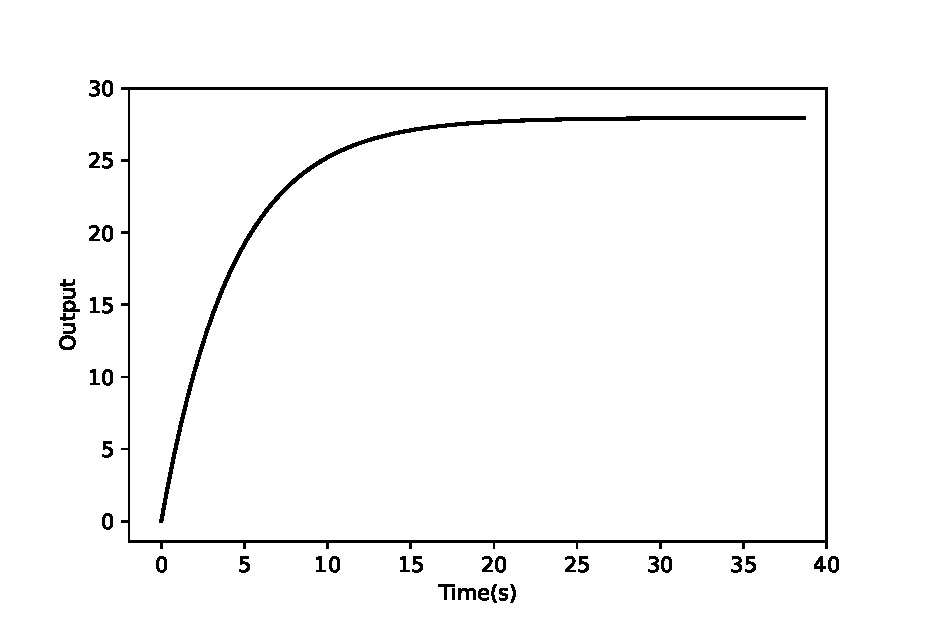
\includegraphics[width=.8\linewidth]{Figures/Question1/EXE_1_SYS_A.eps}  
  \caption{Plot of the system A data.} 
  \label{fig:SYS_A_data}
\end{subfigure}
\begin{subfigure}{.5\textwidth}
  \centering
  % include second image
  \includegraphics[width=.8\linewidth]{Figures/Question1/EXE_1_SYS_B.eps} 
\caption{plot of the system B data.}  
	\label{fig:SYS_B_data}
\end{subfigure}
\end{figure}

%%%%%%%%%%%%%%%%%%%% ITEM 2 OF THE QUESTION:

The graphs provide the information that system A is a first order system and system B is a second order system. Let's start
analysis by data from system A.
\subsection*{System A analysis}
\begin{itemize}
    \item From the data, the final value of the system A output is: $27.94$.
    \item So $63\%$ of its final value is: $17.60$.
    \item Looking into the data $63\%$ of the final value should happened in the following time range:
    \begin{table}[H]
    \centering
    \begin{tabular}{|c|c|}
	\hline    
    Time & Output\\
    \hline
    4.1585 & 17.3237\\
    \hline
    4.3565 &	17.8020\\
    \hline
    \end{tabular}
    \caption{This values defies a range to search the time constant}
    \end{table}
	So, the best time constant going to be found between this two values of time. The constant $\tau$ going to represent the time constant.    
    \item A first order system has the following type:
    \begin{align*}
        G(s) = \frac{K}{\tau s+1}
    \end{align*}
	\item So let's verify how the MSE of the data compare to the simulation of the transfer function varies when $\tau$ changes in the time range between 4.1585 and 4.3565.
	
\begin{figure}[H]
		\centering
		\includegraphics[width=0.4\textwidth]{Figures/Question1/EXE_1_MSE_TIME_CONSTANT.eps}
		\caption{How the error varies as the time variant changes}	
		\label{fig:mse}
\end{figure}
	
The time constant associated with the lowest error is: $\tau=4.2975$. The code \ref{lst:1second} was used to find the time constant associated with he lowest error and plot \ref{fig:mse}. Now some time constants can be calculated.
    \item The settling time: $T_s=\frac{4}{1/\tau}=17.60s$
    \item The rise time: $T_r = \frac{2.2}{1/\tau}=9.45 s$
\end{itemize}

The transfer function of the system is:

\begin{align}
	\label{eq:SYS_A_tf}	
	T_A(s) = \frac{6.503}{s + 0.2327}
\end{align}

The code \ref{lst:1third} was used to calculate the constants and calculate the transfer function of the system.\\
 
The following plot compare the step response of the transfer function in \ref{eq:SYS_A_tf} and the data:  
\begin{figure}[H]
    \centering
    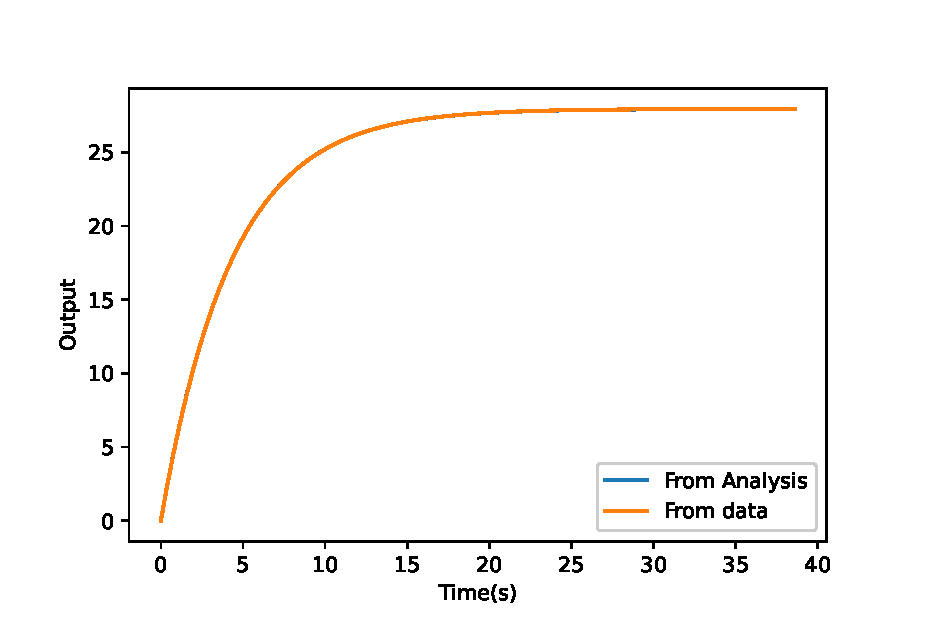
\includegraphics[width=0.5\textwidth]{Figures/Question1/EXE_1_COMPARE_SYS_A.eps}
    \caption{Comparing the step response of the transfer function and the data.}
    \label{fig:SYS_A_COMPARE_PLOT}
\end{figure}
The MSE is: $7.32\times 10^{-6}$, so we can verify that we have a good approximation of the system behavior. 

\subsection*{For the system B}
\begin{itemize}
    \item From the plot, it's possible to assume that the system B is a uderdamped second order system. The general form for this system is:
    \begin{align*}
        G(s)  = \frac{K\omega_n}{s^2+2s\omega_n\zeta+\omega_n^2}
    \end{align*}
    \item Searching in the data the peak time found was: $T_p = 1.0391$
    \item Using the formula:\\ $\%$OS=(max output- final output value)*100/final output value \\the overshoot found was: $OS=36.256\%$
    \item Now that we have the overshoot we can calculate the damping ratio as:
     \begin{align*}
    		\zeta= -\frac{\ln(\%OS/100)}{\sqrt{\pi^2+(\ln(\%OS/100))^2}}
    	\end{align*}
    The damping ration found was $\zeta= 0.307$
    \item So the natural frequency can be calculated as:
    \begin{align*}
    \\\omega_n&=\frac{\pi}{T_p\sqrt{1-\zeta^2}}
    \end{align*} 
    The natural frequency found was: $\omega_n= 3.17$
    \item Now we can use the code \ref{lst:sysB_info} to calculate the following time constants of the system B.
    \item The gain of the system: $K=1.4985$
    \item The rise time of the system is: $T_r=0.423$
    \item The settling time of the system is: $T_s=4.09$
\end{itemize}

In conclusion, the transfer function of the system B:
	\begin{align}
		\label{eq:sys_B_tf}
		T_B(s) = \frac{15.13}{s^2 + 1.953 s + 10.09}
	\end{align}

The code \ref{lst:1sysBstep} was used to plot the step response of the $T_B(s)$ and compare it with the data:
\begin{figure}[H]
    \centering
    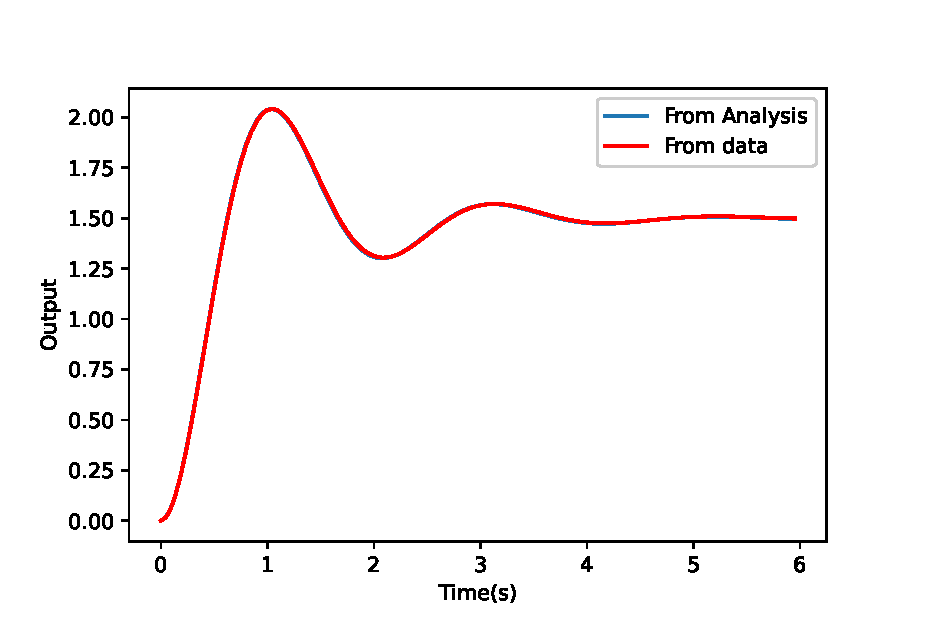
\includegraphics[width=0.5\textwidth]{Figures/Question1/EXE_1_COMPARE_SYS_B.eps}
    \caption{Comparing the step response of the transfer function and the data.}
    \label{fig: MSE_B}
\end{figure}

The mean square error is: $1.827\times10^{-5}$. Based on this, we have a good approximation of the system behavior.
%%%%%%%%%%%%%%%%%%%%%% Exercise 2 %%%%%%%%%%%%%%%%%%%%%%%%%%%%%%%%%
\section*{Exercise 2} 
Consider a system with the transfer function in \eqref{eq: EXE_2_tf}
\begin{align}
	\label{eq: EXE_2_tf}
    G(s) =\frac{\tau s + 1}{(0.1s+1)(0.002s^2+0.02s+1)(s^2+0.1s+1)}
\end{align}
\begin{enumerate}
    	   \item Consider $\tau = 0.5$:
        \begin{itemize}
            \item Find the poles and zeros of the system. Plot them in a zero-pole map and draw some conclusions.
            \item Use a dominant-pole argument to find an equivalent second-order transfer function. Can the zero be neglected in this case? Plot and compare 
            the step responses for system as in \ref{eq: EXE_2_tf} and the second order equivalent one. Explain the differences between the two responses
        \end{itemize}
   		\item Consider $\tau=20$:
    \begin{itemize}
        \item Find the poles and zeros of the system. Plot them in a zero-pole map and draw some conclusions.
        \item Use a dominant-pole argument to find an equivalent second-order transfer function. Can the zero be neglected? Plot and compare the step 
        responses for system as in \ref{eq: EXE_2_tf} and the second order equivalent one. Explain the differences between the two responses.
    \end{itemize}
\end{enumerate}

\section*{Solution}
\subsection*{Consider $\tau = 0.5$}
The zeros and poles of the transfer function are:
\begin{itemize}
    \item For $(0.1s+1)=0$, $s=-10$ is a pole.
    \item For $(0.002s^2+0.02s+1)=0$\\
    The discriminant is $\Delta=-7.6\times10^{-3}$, so we have two complex poles:  $p_1,p_2 = -5\pm21.79j$
    \item For $(s^2+0.1s+1)=0$\\
    The discriminant is $\Delta = -3.99$, so we have two complex poles: $p_1,p_2=-0.05 \pm 0.99j$
    \item For $(0.5s+1)=0$, $s=-2$ is a zero.
\end{itemize}

Therefore, this is the pole zero map:
\begin{figure}[H]
    \centering
    \includegraphics[width=0.5\textwidth]{Figures/Question2/EXE_2_POLE_ZERO_MAP.eps}
    \caption{The poles and zeros of the system}
    \label{fig:exercise2}
\end{figure}
\begin{table}[H]
\centering
\begin{tabular}{|c|c|c|c|c|c|}
\hline
Poles & $-5. +21.79j$&$-5. -21.79j$& $-10$&$-0.05 +0.99j$& $-0.05 -0.99j$\\
\hline
Zeros & -2 & & & &\\
\hline
\end{tabular}
\caption{Table of the poles and zeros of the system.}
\end{table}
There are two poles that are dominant, $p_1,p_2=-0.05 \pm 0.99j$, the other three are more than 5 times bigger, so their impact on the system response is no so big, for this reason they can neglected. Also, the zero can be consider only as a simple gain. To verify what was said, the code \ref{lst:2first} was used to simulate the system step response, the result is in the plot bellow.
\begin{figure}[H]
    \centering
    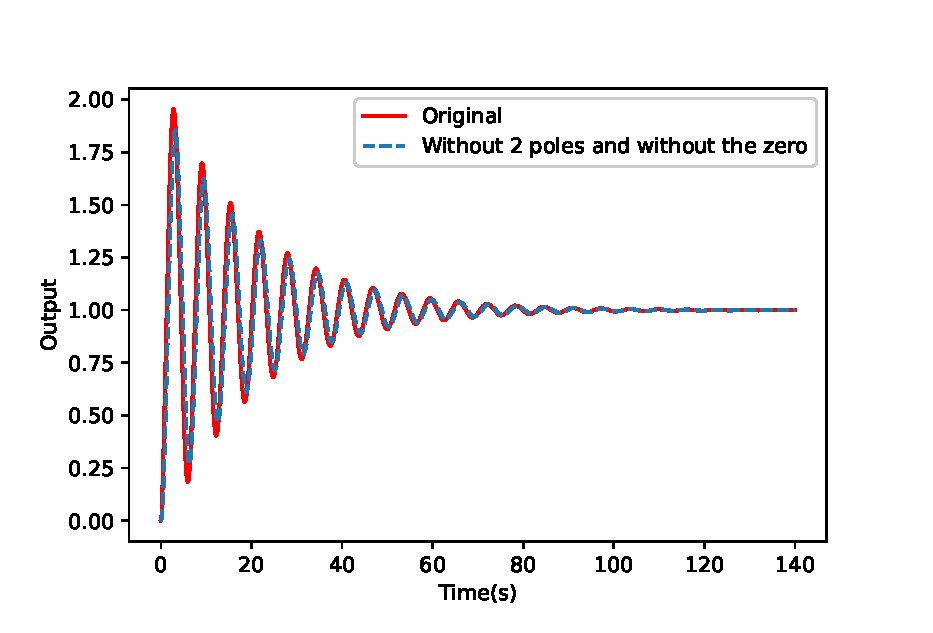
\includegraphics[width=0.5\textwidth]{Figures/Question2/EXE_2_ITEM_2.eps}
    \caption{Compare the original system and the system without the poles.}
    \label{fig:exercise2_item_2}
\end{figure}
The MSE is 0.005. Based on this, we can say that we can approximate the system transfer function to the following second order system:


\begin{align*}
    G(s)=\frac{1}{s^2 + 0.1 s + 1}
\end{align*}
\subsection*{Consider $\tau = 20$}
The poles are the same of the previous system, but there is a different zero:
\begin{itemize}
    \item $(20s+1)=0$,\ $s=0.05$ is a zero.
\end{itemize}

Using the code \ref{lst:2second} the following poles and zero plot were found:

\begin{figure}[H]
    \centering
    \includegraphics[width=0.5\textwidth]{Figures/Question2/EXE_2_POLE_ZERO_MAP_2.eps}
    \caption{The pole and zero map of the transfer function.}
    \label{fig:EXE_2_POLE_ZERO_MAP_2}
\end{figure}

\begin{table}[H]
\centering
\begin{tabular}{|c|c|c|c|c|c|}
\hline
Poles & $-5. +21.79j$&$-5. -21.79j$& $-10$&$-0.05 +0.99j$& $-0.05 -0.99j$\\
\hline
Zeros & -0.05 & & & &\\
\hline
\end{tabular}
\caption{Table of the poles and zeros of the system.}
\end{table}

The zero is close to the dominant poles, we going to see the impact of this in next simulations, and there are 3 poles far from the dominant ones, so they can be neglected, as was presented in the first item. In this sense, we can compare the response of the original system with the response of the following transfer functions:

\begin{align*}
G_1(s) &=  \frac{20 s + 1}{s^2 + 0.1 s + 1}\\
G_2(s) &=  \frac{1}{s^2 + 0.1 s + 1}
\end{align*}

$G_1(s)$ is the transfer function of the system with a zero and the 3 non dominant poles removed. $G_2(s)$ is the transfer function without the 3 non dominant poles and also without the zero. The code \ref{lst:2second} was used to get the following plots:  
\begin{figure}[H]
\begin{subfigure}{.5\textwidth}
  \centering
  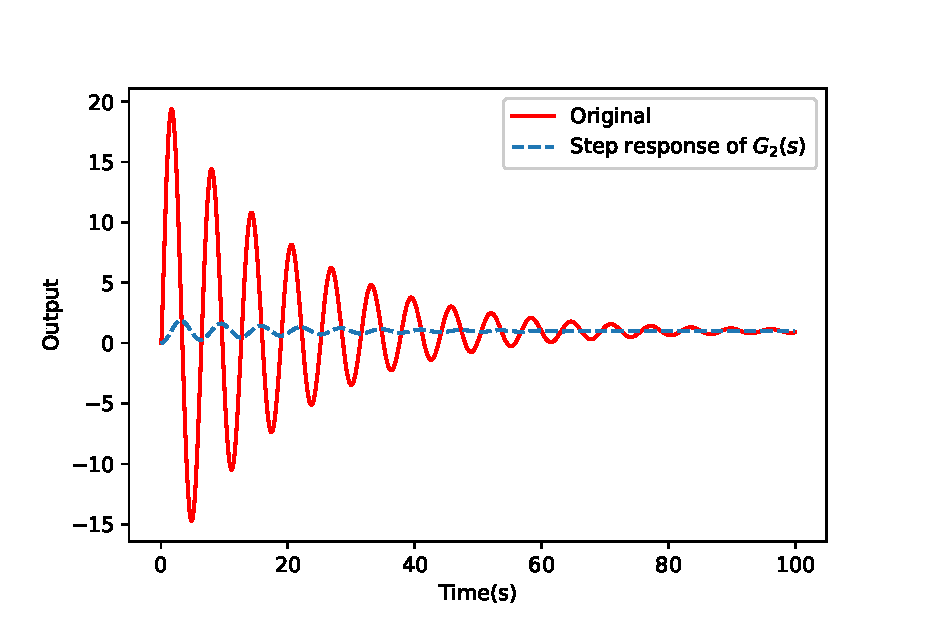
\includegraphics[width=.8\linewidth]{Figures/Question2/EXE_2_ITEM_3.eps}  
  \caption{Comparing $G_2(s)$ step response against the step response of the original transfer function.} 
  \label{fig:EXE_2_ITEM_3}
\end{subfigure}
\begin{subfigure}{.5\textwidth}
  \centering
  % include second image
  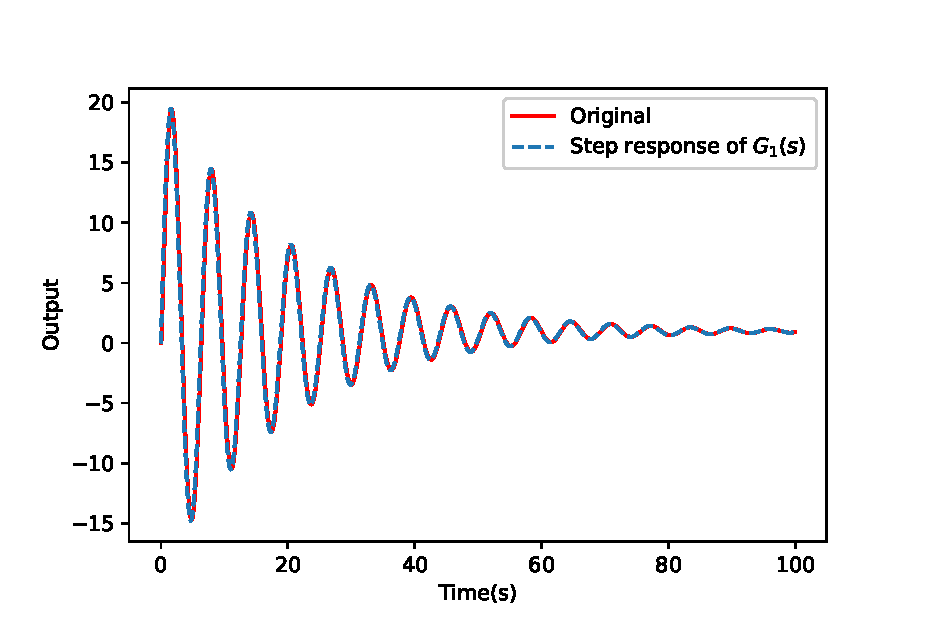
\includegraphics[width=.8\linewidth]{Figures/Question2/EXE_2_ITEM_4.eps} 
\caption{Comparing $G_1(s)$ step response against the step response of the original transfer function.}  
	\label{fig:EXE_2_ITEM_4}
\end{subfigure}
\end{figure}

The plots reflect the relation between the zero near to the origin and the system response, this comes from the fact that the zero near to the dominant poles has an greater impact on the system amplitude compare to the zero far from them, which can be considered as simple gain as was showed in the first item.

In conclusion, $G_1(s)$ represents a better approximation of the system behavior, for this reason we can represent $G(s)$ as:
\begin{align}
\label{eq:Question_2_eq}
G(s) =  \frac{20 s + 1}{
s^2 + 0.1 s + 1}
\end{align}
%%%%%%%%%%%%%%%%%%%%%% Exercise 3 %%%%%%%%%%%%%%%%%%%%%%%%%%%%%%%%%

\section*{Exercise 3}
Given the state-space model in \eqref{eq:Question_3_eq}:
\begin{align}
\label{eq:Question_3_eq}
\begin{cases}
\begin{bmatrix}\dot{x}_1(t)\\
\dot{x}_2(t)\end{bmatrix}= \begin{bmatrix}0 & 1 \\
-5 & -2 \end{bmatrix}\begin{bmatrix}x_1(t) \\x_2(t)\end{bmatrix}+\begin{bmatrix}0\\2\end{bmatrix}u(t)\\
y(t) = \begin{bmatrix} 0 & 1\end{bmatrix}\begin{bmatrix}x_1(t) \\ x_2(t)\end{bmatrix}
\end{cases}\end{align}
\begin{enumerate}
    \item Define the transfer function W (s) of the given system and evaluate the its BIBO stability. Briefly explain the concept of BIBO stability.
    \item Define the Lyapunov's stability of the given system. Briefly explain the concept of stability according to Lyapunov. How does it differ from the BIBO stability?
\end{enumerate}
\section*{Solution}
The transfer function can be calculated as:
    \begin{align}
		\label{eq:system_tf}        
        W(s) =C(sI-A)^{-1}B
    \end{align}
\par Calculating the inverse: 
\begin{align*}
(sI-A)^{-1}=\frac{Adj(sI-A)}{Det{(sI-A)}}
\end{align*}
\par Where $Adj(sI-A)$ is the adjunct matrix of $(sI-A)$. The adjunct matrix is the transpose of the cofactor matrix:
\begin{align*}
Adj(sI-A) = \begin{bmatrix}
s+2 & -5\\
1 & s 
\end{bmatrix}
\end{align*}
\par The inverse of $(sI-A)^{-1}$ is calculated as follows:
\begin{align}
\label{eq:inverse}
(sI-A)^{-1}=\frac{1}{s^2+2s+5}\begin{bmatrix}
s+2 & -5\\
1 & s 
\end{bmatrix}
\end{align}

Using \eqref{eq:inverse} in \eqref{eq:system_tf}:
\begin{align*}
\frac{1}{s^2+2s+5}\begin{bmatrix}
0 & 1
\end{bmatrix}
\begin{bmatrix}
s+2 & -5\\
1 & s 
\end{bmatrix}\begin{bmatrix}
0 \\ 2
\end{bmatrix}=\frac{2s}{s^2+2s+5}
\end{align*}
\par In conclusion:
 \begin{align*}
C(sI-A)^{-1}B=W(s)=\frac{2s}{s^2+2s+5}
\end{align*}

We can find the same answer using the code \ref{lst:3first}.


Calculating the poles of the system:
\begin{align*}
    s^2+2s+5&=0\\
    \Delta&=4-20=-16\\
    p_1,\ p_2&=-1 \pm 2j
\end{align*}


Using \ref{lst:3pzmap} we get the following:
\begin{figure}[H]
    \centering
    \includegraphics[width=0.5\textwidth]{Figures/Question3/EXE_3_POLE_ZERO_MAP.eps}
    \caption{The poles and zeros of the transfer fucntion. Look the each poles is in the left hand side of the system.}
    \label{fig:POLE_ZERO_MAP_3}
\end{figure}

The transfer function of the system has 2 poles in the left hand side of the Argan-Gauss plan. As a result, the exponential terms in the system time response going to have an decreasing behavior, so as the time pass the system response goes to tend to a equilibrium point. For this reason, a bounded input can only deliver the system response for a bounded response, This is also called a BIBO stable system. We can verify this by seen the step response of the system. The code used to perform this plot was \ref{lst:3second}.
\begin{figure}[H]
    \centering
    \includegraphics[width=0.5\textwidth]{Figures/Question3/EXE_3_SYS_OUTPUT.eps}
    \caption{The system  step response.}
    \label{fig:EXE_3_STEP_RESPONSE}
\end{figure}
\subsection*{Lyapunov stability of the system}
For a linear system we can divide the system response in the input response and the state response. The first one is related on how the system behavior changes due to the interaction of some manipulated variable. The other one can be seen as the effect of the initial states variables values in the system response. This is exemplify by the following equation:
\begin{align}
x(t) = e^{At}x_0+\int_0^\tau e^{A(t-\tau)}Bu(\tau)d\tau  
\end{align}
Therefore, the state response can be considered to be only:
\begin{align}
x(t) =  e^{At}x_0
\end{align}

Based on the previous equation, the system can go from some initial position to some $x(t)$, that could or not be near to an equilibrium point of the system. This is the context that the Lyapunov stability take place, because Lyapunov verifies if a system can naturally goes from some point in the space back to the equilibrium point. In this context, naturally means that the system is driving by the relation of the states. There are many examples of this kind of system, for example the equilibrium in natural chemical reactions, where there are reagents that are consumed and other are produced until an stabilization. In the other hand there are some system that are not naturally drive, for example the stick up is an equilibrium position for a stick, but it can not be drive to the up position naturally it tends to move far from this point.

In this context, Lyapunov call a system that can goes from an initial state to the equilibrium point as asymptotically stable, if the system tends to a point that is not the equilibrium the system is said to be marginally stable. Mathematically the Lyapunov stability can be introduced as follows: 


\begin{itemize}

\item The system is marginally stable if and only if all eigenvalues of A have zero or negative
real parts and those with zero real parts are simple roots of the minimal polynomial of A .

\item The system is asymptotically stable if and only if all eigenvalues of A have negative real parts.

\end{itemize}

In the system represented by \eqref{eq:Question_3_eq} the code \ref{lst:3_eigenvalues} was used to verify the system eigenvalues, the result are in the table below:

\begin{table}[H]
\centering
\begin{tabular}{|c|c|c|}
\hline
Eigenvalue & Real part & Imaginary part\\
\hline
$\lambda_1$&-1& 2i\\ 
\hline
$\lambda_2$& -1& -2i\\
\hline
\end{tabular}
\caption{The eigenvalues of the system}
\end{table}

In conclusion, based on the previous table the system is said to be asymptotically stable. The code \ref{lst:3_lyapunov} creates the following plot, that plot show how the system goes from a different initial state to zero when there is no input applied.
\begin{figure}[H]
\centering
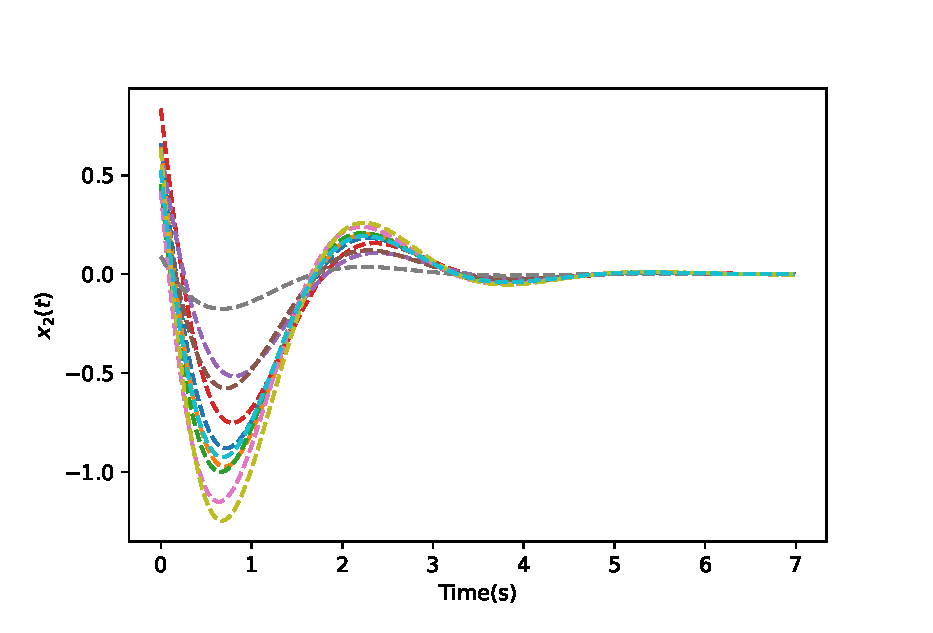
\includegraphics[width=0.5\textwidth]{Figures/Question3/EXE_3_SYS_LYAPUNOV.eps}
\caption{The system state response for different initial conditions}
\end{figure}
%%%%%%%%%%%%%%%%%%%%%% Exercise 4 %%%%%%%%%%%%%%%%%%%%%%%%%%%%%%%%%
\section*{Exercise 4} 
For the unit feedback system in figure , G(s) is given as:
\begin{align*}
    G(s) =\cfrac{s+4}{s(s^2+3.2s+2.4)} 
\end{align*}
\begin{figure}[H] \begin{center}
\includegraphics [width=0.5\textwidth] {Figures/FromMichela/Question4_Figure_1.pdf} \vskip-0.4cm
\caption{Feedback system used in Exercise 4.}
\label{fig:ex4}
\end{center}
\end{figure}
\begin{enumerate}
    \item Use the Routh-Hurwitz criterion to define:
    \begin{itemize}
        \item The range of K that provides stability to the closed-loop system.
        \item The range of K that makes the system oscillate.
    \end{itemize}
    \item Plot and discuss the step responses for stable and oscillatory values of K.
\end{enumerate}
\section*{Solution}
The transfer function of the closed loop system can be calculated as:
\begin{align*}
    \frac{R(s)}{C(s)}=T(s)=\frac{KG(s)}{1+KG(s)}
\end{align*}

Replacing the G(s), the following transfer function was found:
\begin{align*}
    T(s) = \frac{K(s+4)}{s^3+3.2s^2+2.4s+K(s+4)}
\end{align*}

Let's verify how is the Routh table of the system:
\begin{table}[H]
    \centering
    \begin{tabular}{|c|c|c|}
	\hline    
    $s^3$  & $1$ & $(2.4+K)$  \\
    \hline
    $s^2$    &  3.2 & 4K  \\
    \hline
    $s$ & $(3.2(2.4+K)-4K)/3.2$ &0 \\
    \hline
    $s^0$ & 4K &0 \\
    \hline
    \end{tabular}
    \caption{Routh table of the transfer function}
    \label{tab:EXE_2_ROUTH_TABLE_1}
\end{table}

To avoid the poles in the right hand side of the Argan-Gauss plane the table can't have signal changes in the first column, so:
\begin{itemize}
    \item $\frac{(3.2(2.4+K)-4K)}{3.2}>0$. Then, $9.6>K$. So, the value of K for the system be stable is: $0<K<9.6$.
    \item The following plot show how the poles of the system varies as the value of the K keeps on the range and when the values of the K goes out of the range:
    \vspace{-1em}
    \begin{multicols}{2}
    \begin{figure}[H]
        \centering
        \includegraphics[width=0.5\textwidth]{Figures/Question4/EXE_4_ITEM_1.eps}
        \caption{Poles when 9.6>K>0 }
        \label{fig:EXE_2_POLES_LHP}
    \end{figure}
   \columnbreak
   
    
    \begin{figure}[H]
        \centering
        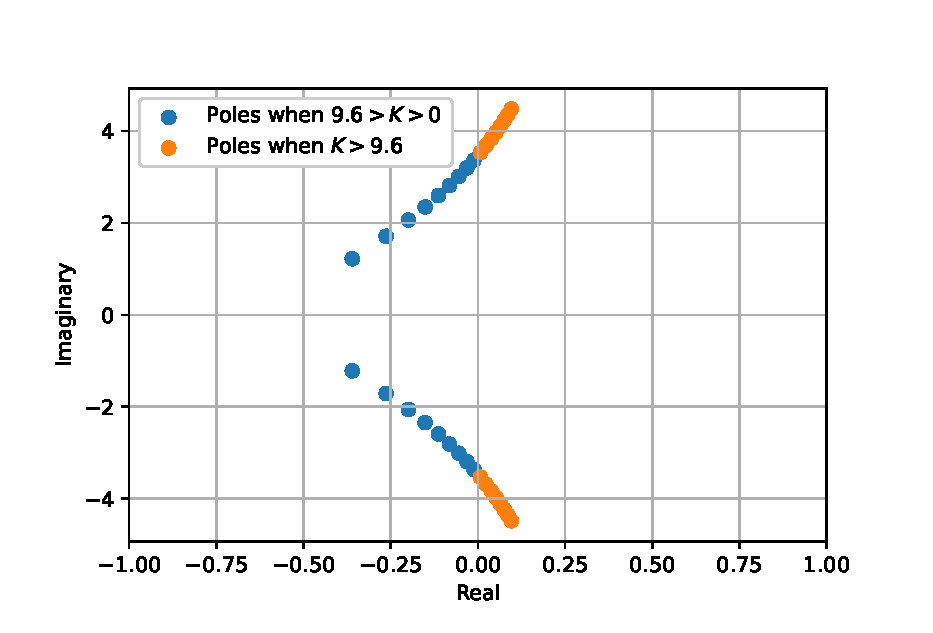
\includegraphics[width=0.5\textwidth]{Figures/Question4/EXE_4_ITEM_2.eps}
        \caption{Showing the poles when $K>9.6$}
        \label{fig:EXE_2_POLES_RHP}
    \end{figure}
    \end{multicols}
\end{itemize}

When $K =9.6$ we going to have the following situation in the Routh table:
\begin{table}[H]
    \centering
    \begin{tabular}{|c|c|c|}
	\hline    
    $s^3$  & $1$ & $(2.4+K)$  \\
    \hline
    $s^2$    &  3.2 & 4K  \\
    \hline
    $s$ & 0 &0 \\
    \hline
    $s^0$ & ? &0 \\
    \hline
    \end{tabular}
    \caption{Routh table of the transfer function}
    \label{tab:EXE_2_ROUTH_TABLE_2}
\end{table}
To by-pass this situation it's necessary to use the derivative of the even polynomial:
\begin{align*}
    p(s)=3.2s^2+4*(9.6)&=0\\
    \frac{d p(s)}{ds}&=6.4s
\end{align*}

So, we replace the 0 for 6.4:
\begin{table}[H]
    \centering
    \begin{tabular}{|c|c|c|}
	\hline    
    $s^3$  & $1$ & $(2.4+K)$  \\
    \hline
    $s^2$    &  3.2 & 4K  \\
    \hline
    $s$ & 6.4 &0 \\
    \hline
    $s^0$ & 4*9.6 &0 \\
    \hline
    \end{tabular}
    \caption{Routh table of the transfer function}
    \label{tab:EXE_3_ROUTH_TABLE_3}
\end{table}

The row of zeros is caused by an even polynomial of degree 2, which has symmetric roots. The missing of signal changes bellow the row of zeros gives the information that the even polynomial has no roots in the RHP, so to keep the symmetry of its roots they need to be in the imaginary axis. To show this the code \ref{lst:4PZMAP} was used to plot the poles and zero map of the system.
 
\begin{figure}[H]
        \centering
        \includegraphics[width=0.5\textwidth]{Figures/Question4/EXE_4_ITEM_3.eps}
        \caption{Showing the poles when $K=9.6$.}
        \label{fig:EXE_POLES_MARGINALLY}
    \end{figure}

The following table summary the result found:
\begin{table}[H]
\centering
\begin{tabular}{|c|c|}
\hline
$K \in(-\infty,0)$& The system is unstable.\\
\hline
$K \in (0,9.6)$ & The system is stable\\
\hline
$K =9.6$ & The system is marginally stable\\
\hline
$K \in (9.6,+\infty)$& The system is unstable\\
\hline
\end{tabular}
\caption{How the stability varies as K varies. }
\end{table}
To exemplify what was said in the last sections the following plot was made varying the value of K in the range of (0, 9.6). It's is possible to verify that the system response goes to stabilize, but when K increases in the range the amplitude and time for stabilization increases. This is a reflect of the approximation of the poles to the imaginary axis which represents a reduction of the negative real part and a increases of the imaginary part.
\begin{figure}[H]
\centering
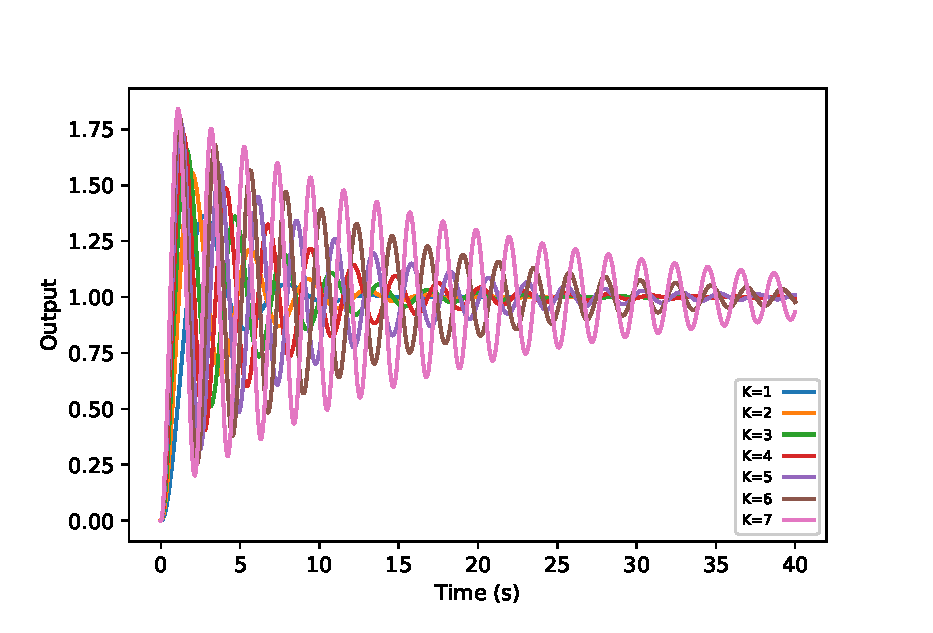
\includegraphics[width=0.5\textwidth]{Figures/Question4/EXE_4_MULTIPLE_PLOTS.eps}
\caption{Step response of the closed loop system for different values of K.}
\end{figure}
Now when K is equal to 9.6, the response does not goes to stabilize, but it not going to infinity. The response is a pure oscilation with a constant amplitude, this reflects the poles that are in the imaginary axis.
\begin{figure}[H]
\centering
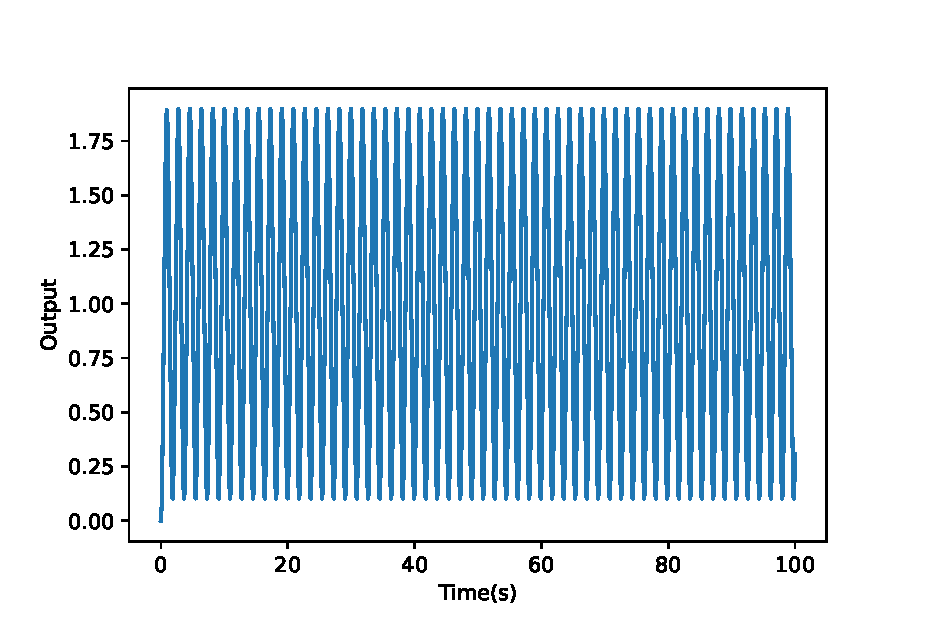
\includegraphics[width=0.5\textwidth]{Figures/Question4/EXE_4_ITEM_5}
\caption{Step response of the system when K=9.6}
\end{figure}
%%%%%%%%%%%%%%%%%%%%%%% Exercise 5 %%%%%%%%%%%%%%%%%%%%%%%%%%%%%%%%
\section*{Exercise 5}
A unity feedback system has the forward transfer function given by:
\begin{align}
    G(s) = \frac{K(s+7)}{s(s^3+25s^2+196s+480)} 
\end{align}
\begin{enumerate}
    \item Evaluate the system type.
    \item Find the value of K to yield a $1\%$ error in steady-state for an input of 0.1t.
    \item Find the static error constants for the value of K found in point (2) of this exercise.
    \item Verify the stability of your system and plot its step response.
\end{enumerate}
\section*{Solution}

The system is type 1, because the number of integrators in the forward path is 1.

The error in the s domain is given by:
\begin{align*}
    \mathcal{L}\{e(t)\}&=E(s)=Y(s)-R(s)\\
    E(s)G(s) &= Y(s)\\
    \frac{R(s)G(s)}{1+G(s)}&=Y(s)\\
    E(s) &= R(s)\frac{1}{1+G(s)}
\end{align*}

For a stable system, the final value theorem can be used to calculate the stationary error. I going to suppose that the system is stable, and them calculate K, after find it I going to check using the Routh Table if for this value the system is stable.

\begin{align}
    e(\infty)=\lim_{s\rightarrow 0}sE(s)
\end{align}

So, for $r(t) = 0.1 t$:

\begin{align*}
e(\infty)=\lim_{s \rightarrow 0}s\frac{0.1}{s^2}\frac{1}{1+G(s)}=\frac{0.1}{\lim_{s\rightarrow 0}sG(s)}=\frac{480*0.1}{7K}\\
\end{align*}

So for $e(\infty)=0.01$. $K=\frac{480*0.1}{0.01*7}=685.71$.

Now, let's certify that the system is stable:
\begin{align*}
    T(s) = \frac{G(s)}{1+G(s)}=\frac{K(s+7)}{K(s+7)+s(s^3+25s^2+196s+480)}=\frac{685.71(s+7)}{s^4+25s^3+196s^2+1165.71s+4799.97}
\end{align*}

	After that we can create the Routh table:
\begin{table}[H]
    \centering
    \begin{tabular}{|c|c|c|c|}
	\hline    
    $s^4$  & 1 & 196 & 4799.97\\
    \hline
    $s^3$ & 25 & 1165.71 & 0\\
    \hline
    $s^2$ & 149.37 & 4799.97&0\\
    \hline
    $s^1$ & 365.34 &0& 0\\
    \hline
    $s^0$ & 4799.97 & 0 & 0\\
    \hline
    \end{tabular}
    \caption{The Routh table of the system. There are no signals change in the first column, so the system is stable}
    \label{tab:my_label}
\end{table}
From the Routh table we can verify that the system is stable, because there is no signal change in the first column. To showing this explicit the pole zero 
map was plot:
\begin{figure}[H]
    \centering
    \includegraphics[width=0.5\textwidth]{Figures/Question5/EXE_5_ITEM_4.eps}
    \caption{The poles of the closed loop system}
    \label{fig:my_label}
\end{figure}
Using \ref{lst:5third} we got the following plot for the system step response.
\begin{figure}[H]
    \centering
    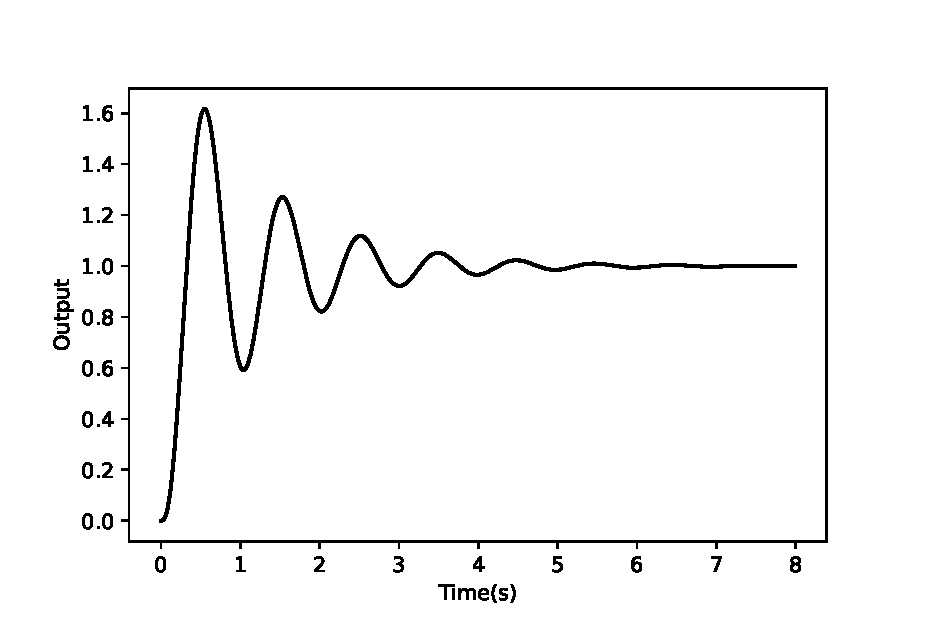
\includegraphics[width=0.5\textwidth]{Figures/Question5/EXE_5_ITEM_3.eps}
    \caption{The step response of the system}
    \label{fig:my_label}
\end{figure}
Then, the static error constants were calculated.
\begin{itemize}
    \item Position Constant: $K_p = \lim_{s\rightarrow 0}G(s)=\infty$. This value comes from the fact that the forward path transfer function has 1 pole in the origin, so when s goes to zero, G(s) goes to tend to the infinity. It gives the information that for a constant input, the error in the stationary goes to be zero, since the error is:
\begin{multicols}{2} 
    \begin{align*}
    e(\infty)=\lim_{s\rightarrow 0}\frac{1}{1+G(s)}=0
    \end{align*}
    \columnbreak
    \begin{figure}[H]
    \centering
    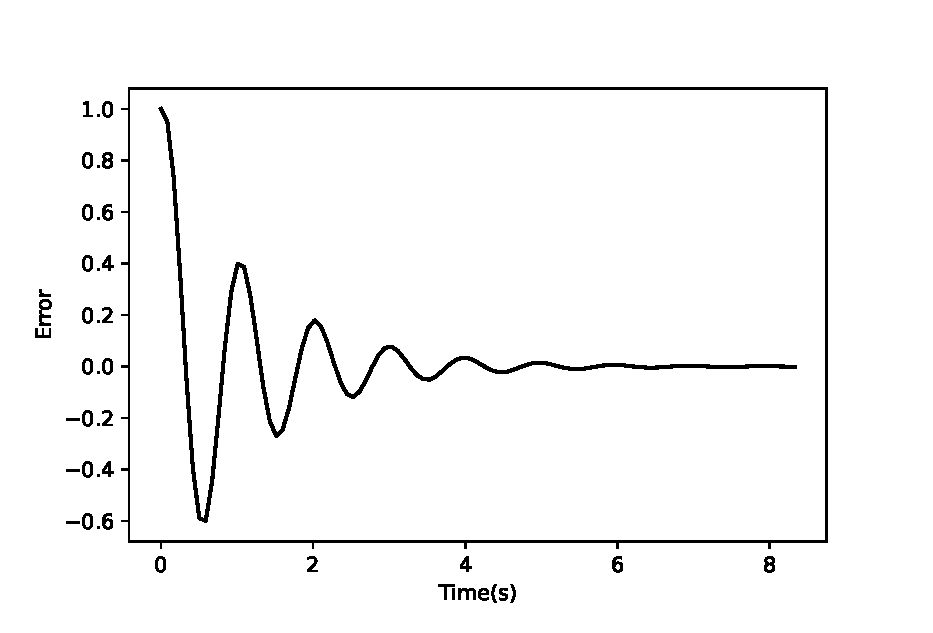
\includegraphics[width=0.5\textwidth]{Figures/Question5/EXE_5_step_error.eps}
    \caption{The error for a step input}
    \end{figure}
\end{multicols}
	\item Velocity Constant:   $K_v = \lim_{s\rightarrow 0}sG(s)=\frac{7K}{480}=\frac{0.1}{0.01}=10$. This values shows that for a input that increases in a linear relation with the time such as the ramp, the system goes to have some constant error. For the $r(t) = 0.1t$
\begin{multicols}{2}	
	\begin{align*}
    e(\infty)=\lim_{s\rightarrow 0}\frac{0.1}{sG(s)}=\frac{0.1}{K_v}=\frac{0.1}{10}=0.01
    \end{align*}
    \columnbreak		
	\begin{figure}[H]
    \centering
    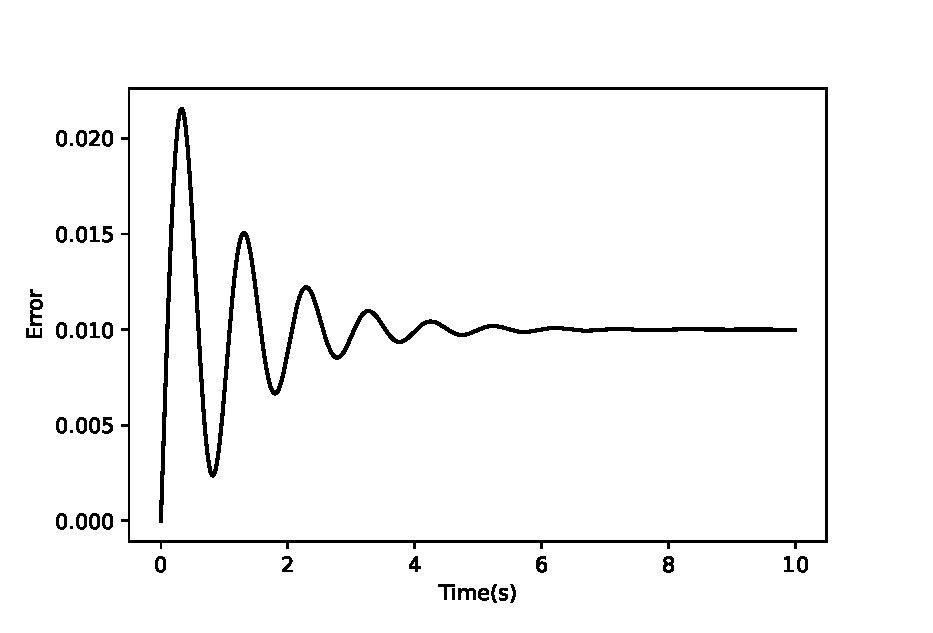
\includegraphics[width=0.5\textwidth]{Figures/Question5/EXE_5_ITEM_2.eps}
    \caption{The error for $r(t)=0.1t$.}
    \label{fig:EXE_error}
\end{figure}
\end{multicols}
	\item Acceleration constant $K_a = \lim_{s\rightarrow 0}s^2G(s)=0$. This value comes from the fact that G(s) does not have enough poles to cancel the $s^2$, so this value goes $K_a$ goes to zero. For a $r(t)=t^2$ the error is:
	\vspace{-1em}	
	\begin{multicols}{2}	
	\begin{align*}
    e(\infty)=\lim_{s\rightarrow 0}\frac{1}{s^2G(s)}=\frac{1}{K_a}=\infty
    \end{align*}
    \columnbreak	
	\begin{figure}[H]
    \centering
    \includegraphics[width=0.5\textwidth]{Figures/Question5/EXE_5_parabola_error.eps}
    \caption{The error for a parabola}
    \label{fig:EXE_error}
\end{figure}
\end{multicols}
\end{itemize}
%%%%%%%%%%%%%%5 EXERCISE 6 %%%%%%%%%%%%%%%%%%%%%%%%%5
\section*{Exercise 6}
\begin{figure}[H] \begin{center}
\includegraphics [width=0.5\textwidth] {Figures/FromMichela/Question6_Figure_1.pdf} \vskip-0.4cm
\caption{Feedback system used in Exercise 6}
\label{fig:ex6}
\end{center}
\end{figure}

The Figure \ref{fig:ex6} represents a cascade control system of the temperature, $Y_1$ , in a small room which
is achieved by adjusting the hot/cold water flow, $Y_2$ , adjusted by an inner control loop (coloured in Figure \ref{fig:ex6}). 

The relationship between the room temperature and the water low rate can be represented with the transfer function $G_{p1}$ , whereas $G_{p2}$ corresponds to the conditioning unit. $G_{c2}$ represents the water flow rate controller and $G_{c1}$ keeps the room temperature at the desired set-point by defining the needed water flow rate. $G_{m1}$ and $G_{m2}$ correspond to the temperature and flow rate measuring devices, respectively.

The disturbances can influence the system: $D_1$ represents unwanted changes in the water
pressure inside the pipes and might affect $Y_2$ and $D_2$ represents possible variations in the
external temperature and might affect $Y_1$.
\begin{enumerate}
    \item Assuming $D_1 = D_2 = 0$, find the input-output transfer functions for the inner and outer loops: $Y_1/Y_{sp1}$ and $Y_2/Y_{sp2}$.
    \item Assuming $Y_{sp1} = D_1 = 0$, find the disturbance-output transfer functions: $Y_1 /D_2$
    \item Assuming $Y_{sp1} = D_2 = 0$, find the disturbance-output transfer functions: $Y_2/D_1$.
    \item Define the characteristic equation of the cascade control system in Figure 2 and
analyses the stability of the system.
\item For $K_{c2} = 1$, verify whether is possible or not simplify the input-output $\frac{Y_1(s)}{Y_{sp1}}$
representation found in point (1) of this exercise.
\item Compare the two cases (with and without simplification) by plotting the response
of the system to a unit step input. From the plot, identify the steady-state value,
the percentage overshoot and settling time in the two cases.
\end{enumerate}

\begin{align*}
\begin{split}
G_{p1}(s)= & \cfrac{K_{p1}}{(1+\tau_{p1,1}s)(1+\tau_{p1,2}s)}=\cfrac{0.1}{1000s^2+70s+1}\\ 
G_{p2}(s)=& \cfrac{K_{p2}}{1+\tau_{p2}s}=\cfrac{1}{1+10s}\\ 
G_{c1}(s)=& K_{c1}=100  \\
G_{c2}(s)= & K_{c2}\cfrac{1+\tau_{c2}s}{s}=K_{c2}\cfrac{1+100s}{s} \\
G_{m1}(s)=&  1; \quad G_{m2}(s)= \cfrac{K_{m2}}{1+\tau_{m2}s}=\cfrac{1}{1+s}\\
G_{d1}(s)=&  1; \quad G_{d2}(s)= 1
\end{split}
\end{align*}

\section*{Solution}

First, let's have a look of the system inside:

\begin{align*}
(Y_{sp2}-G_{m2}Y_2)&=E_2(s)\\
E_2(s)G_{c2}G_{p2}&=Y_2(s)\\
(Y_{sp2}-G_{m2}Y_2)&=\frac{Y_2(s)}{G_{c2}G_{p2}}\\
Y_{sp2}(s)G_{c2}(s)G_{p2}(s)&=Y_2(s)(1+G_{m2}(s)G_{c2}(s)G_{p2}(sc))
\end{align*}

So, the transfer function $H_2(s)$:

\begin{align*}
    H_2(s) = \frac{Y_2(s)}{Y_{sp2}(s)}=\frac{G_{c2}G_{p2}}{1+G_{m2}G_{c2}G_{p2}}=\frac{K_{c2}(1+100s)(s+1)}{s(s+1)(1+10s)+K_{c2}(1+100s)}
\end{align*}

For $K_{c2}=1$:

\begin{align}
	\label{eq: EQ_6_EXE}    
    H_2(s)=\frac{100 s^2 + 101 s + 1}{10 s^3 + 11 s^2 + 101 s + 1}
\end{align}

Now for the system outside:

\begin{align*}
    Y_{sp1}(s)-G_{m1}Y_1(s)&=E_1(s)\\
    E(s)G_{c1}H_2(s)G_{p1}&=Y_1(s)\\
    (Y_{sp1}(s)-G_{m1}Y_1(s))G_{c1}H_2(s)G_{p1}&=Y_1(s)
\end{align*}

So the transfer function $H_1(s)$

\begin{align*}
    H_1(s) &= \frac{Y_1(s)}{Y_{sp1}(s)} =\frac{G_{c1}(s)H_2(s)G_{p1}(s)}{1+G_{m1}(s)G_{c1}(s)H_2(s)G_{p1}(s)}\\H_1(s)&=\frac{10K_{c2}(1+100s)(s+1)}{(1000s^2+70s+1)(s(s+1)(1+10s)+K_{c2}(1+100s))+10K_{c2}(1+100s)(s+1)}\\
	H_1 &=\frac{10K_{c2}(1+100s)(s+1)}{10^4s^5+1.1710^4s^4+(1780+10^5K_{c2})s^3+(81+910^3K_{c2})s^2+(1+1180K_{c2})s+11K_{c2}}
\end{align*}

For $K_{c2}=1$:

\begin{align}
\label{eq:EQ_H1(s)}    
    H_1(s)=\frac{1000 s^2 + 1010 s + 10}{
  10000 s^5 + 11700 s^4 + 101780 s^3 + 9081 s^2 + 1181 s + 11}
\end{align}

Now for $Y_{sp1}=D_{1}=0$, the transfer function of the disturbance-output $Y_1(s)/D_2(s)=H_3(s)$.

\begin{align*}
-Y_1(s)G_{m1}G_{c1}H_2(s)G_{p1}(s)+D_2 &= Y_1(s)\\
\frac{Y_1(s)}{D_2(s)}&=\frac{1}{1+G_{m1}G_{c1}H_2(s)G_{p1}(s)}\\
\end{align*}

For the $K_{c2}=1$ the transfer function $H_3(s)$ is:
\begin{align}
H_3(s)&=\frac{10^4 s^5 + 1.17\times10^4 s^4 + 1.018\times10^5 s^3 + 8081 s^2 + 171 s + 1}{10^4s^5 + 1.17\times10^4s^4 + 1.018\times10^5 s^3 + 9081 s^2 + 1181 s + 11}
\end{align}

Now, the disturbance-output transfer function $Y_2(s)/D_1(s)=H_4(s)$:

\begin{align*}
D_1(s)-Y_2(s)G_{m2}G_{c2}G_{p2}&=Y_2(s)\\
D_1(s)&=Y_2(s)G_{m2}G_{c2}G_{p2}+Y_2(s)\\
H_4(s)&=\frac{Y_2(s)}{D_2(s)}=\frac{1}{G_{m2}G_{c2}G_{p2}+1}
\end{align*}

For $K_{c2}=1$:
\begin{align}
H_4(s)&=\frac{10 s^3 + 11 s^2 + s}{10 s^3 + 11 s^2 + 101 s + 1}
\end{align}

From $H_1(s)$, the characteristic polynomial 
\begin{align*}
p(s) &= 10^4s^5+1.1710^4s^4+(1780+10^5K_{c2})s^3+(81+910^3K_{c2})s^2+(1+1180K_{c2})s+11K_{c2}
\end{align*}

To simplify a little bit the analysis, I choose to make the following approximations:
\begin{align*}
(1780+10^5K_{c2})&\approx10^5K_{c2}\\
(81+910^3K_{c2})&\approx910^3K_{c2}\\
(1+1180K_{c2})&\approx1180K_{c2}
\end{align*}
\begin{table}[H]
\centering
\begin{tabular}{| c | c| c | c|c|}
	\hline	
	$s^5$&$10^4$  & $10^5K_{c2}$ & $1180K_{c2}$ \\
    \hline
    $s^4$&$11700$& $910^3K_{c2}$ & $11K_{c2}$\\
    \hline
    $s^3$ & $92307.69K_{c2}$&$1170.59K_{c2}$&0\\
    \hline
    $s^2$&$910^3K_{c2}+148.37=\sigma_1$& $11K_{c2}$ &0\\
    \hline
    $s^1$ & $(\sigma_1*1170.59K_{c2}-11K_{c2}*92307.69K_{c2})/\sigma_1$&0 &0\\
    \hline
    $1$ & $11K_{c2}$ & 0 & 0\\
	\hline   
    \end{tabular}
    \caption{Routh Table of the exercise.}
    \label{tab:routh_table_ex_6}
\end{table}
To not have signal changes in the first column it's necessary that:
\begin{align*}
910^3K_{c2}+148.37>0 \therefore K_{c_2}>-0.0164\\
(\sigma_1*1170.59K_{c2}-11K_{c2}*92307.69K_{c2})>0 \therefore K_{c2}>-0.01824
\end{align*}

From this approximate simple analysis, it's possible to say that for all positive values of $K_{c2}$ the system is stable.
\subsection*{For $K_{c1}=1$}
The transfer function is presented in the equation \ref{eq:EQ_H1(s)}. The poles of the system are:
\begin{multicols}{2}
\begin{table}[H]
\centering
\begin{tabular}{|c|c|c|}
\hline
Poles & Real & Imaginary \\
\hline
$s_1$ & -0.5405 & + 3.1270i\\
\hline
$s_2$&  -0.5405 & - 3.1270i\\
\hline
$s_3$&  -0.0395 & 0.1356i\\
\hline
$s_4$&  -0.0395 & - 0.1356i\\
\hline
$s_5$&  -0.0100 & + 0.0000i\\
\hline
\end{tabular}
\caption{The poles of the system}
\end{table}
\columnbreak
\begin{table}[H]
\centering
\begin{tabular}{|c|c|c|}
\hline
Zeros & Real & Imaginary\\
\hline
$Z_1$ &  -1.0000 & 0 \\
\hline
$Z_2$ & -0.0100 & 0\\
\hline
\end{tabular}
\caption{The zeros of the system}
\end{table}
\end{multicols}
\begin{figure}[H]
\centering
\includegraphics[width=0.5\textwidth]{Figures/Question6/EXE_6_pzmap.eps}
\caption{Pole zero map of the system}
\end{figure}

There is a zero pole cancellation, an also there are some poles that are much far from the origin as the dominant poles,$-0.0395 \pm - 0.1356j$, we can verify this looking into the poles of the system. So the system can be represented by a second order transfer function:
\begin{align*}
T(s) = \frac{K}{(s+0.0395+0.0968j)(s+0.0395-0.0968j)}
\end{align*}

The value of K can be calculated using the final value theorem and the original system simulation, using the code \ref{lst:6first} we can verify that $K=0.0099$. Then it's possible to approximate the system to the following transfer function:
\begin{align}
T(s) &=\frac{0.01}{(s+0.0395+0.0968j)(s+0.0395-0.0968j)}
\end{align}

The plot below shows how the step response of the system is near to the step response of $T(s)$.
\begin{figure}[H]
\centering
\includegraphics[width=0.5\textwidth]{Figures/Question6/EXE_6_FINAL_PRINT.eps}
\end{figure}
The MSE is 0.0026, so we can have this as system approximation. Using the same formulas of the second question and with the data from the step response the code \ref{lst:6_info} was used to give the information ahead.
\begin{multicols}{2}
For the transfer function $H_1(s)$:
\begin{itemize}
\item Settling time: 101.17463342822805
\item Peak Time: 32.45
\item The natural frequency:  0.10457478294286249
\item The damping ratio: 0.3780605657969098
\item Overshoot 27.722376800944076
\item The gain of the system:  0.9150664921824592
\end{itemize}
\columnbreak

Using the same code for $T(s)$
\begin{itemize}
\item Settling time: 98.85555378922112
\item Peak Time: 31.52
\item The natural frequency:  0.10757013178822733
\item The damping ratio: 0.37615532761901993
\item Overshoot 27.93202729653574
\item The gain of the system:  0.9091545682955544
\end{itemize}
\end{multicols}


\newpage
\section*{Appendix}
\appendix 
\subsection*{Homework Notebook}
\par There is a python notebook for the homework: \href{https://colab.research.google.com/drive/1j09ifwj77xrI9G4FtcCSJtw4kdnd3njG}{Notebook with the answer}. The notebook has the following advantages:
\begin{itemize}
\item Each code is separated for each exercise.
\item The notebook already has all modules used in this homework installed.
\end{itemize}


\section{Source code for exercise 1}

\begin{lstlisting}[caption={Code to load the data and plot.}\label{lst:1first}]
import pandas as pd
import matplotlib.pyplot as plt
## Loading the data.
sys_A_df = pd.read_csv('sysA.csv')# You need to have sysA.csv.
sys_B_df = pd.read_csv('sysB.csv')# You need to have sysB.csv.

## Plot the response for the first system
plt.plot(sys_A_df['Tempo'],sys_A_df['Output'],'k')
plt.grid('on')
plt.xlabel('Time(s)')
plt.ylabel('Output')
plt.ylim(top=30)
plt.xlim(right=40)
plt.show()

### Plot the response for the second system.
plt.plot(sys_B_df['Tempo'],sys_B_df['Output'],'k')
plt.grid('on')
plt.xlabel('Time (s)')
plt.ylabel('Output')
plt.savefig('EXE_1_SYS_B.eps',format='eps')
plt.show()
\end{lstlisting}

\begin{lstlisting}[caption={Code to verify the MSE for different values of time constant.}\label{lst:1second}]
import numpy as np
from sklearn.metrics import mean_squared_error as mse
import matplotlib.pyplot as plt 
import pandas as pd
sys_A_df = pd.read_csv('sysA.csv')# You need to have sysA.csv.
Final_Value=sys_A_df['Output'].values[-1]
time_constant_output = 0.63*Final_Value

initial_value_time = (sys_A_df.loc[sys_A_df['Output']<=time_constant_output]['Tempo'].values[-1])
final_value_time  = (sys_A_df.loc[sys_A_df['Output']>=time_constant_output]['Tempo'].values[0])

time_constant_range=np.arange(initial_value_time,final_value_time,0.001)
error_vector =[]
for time_constant in time_constant_range: 
    a = 1/time_constant
    sys_A_tf = tf([Final_Value*a],[1,a])
    y_out,T=step(sys_A_tf,np.arange(0,196*0.198,0.198))
    error= mse(sys_A_df['Output'],y_out)
    error_vector.append(error)

time_constant=time_constant_range[error_vector.index(min(error_vector))]
a = 1/time_constant

plt.plot(time_constant_range,error_vector)
plt.ylabel('MSE')
plt.xlabel('Time constant (s)')
plt.savefig('EXE_1_MSE_TIME_CONSTANT.eps',format='eps')
plt.show()
\end{lstlisting}

\begin{lstlisting}[caption={Code to find the system A transfer function and constant values.}\label{lst:1third}]
sys_A_tf = tf([Final_Value*a],[1,a])

step_info_sys_A = stepinfo(sys_A_tf)
settling_time = 4/a
rise_time = 2.2/a 

print("Final values (Gain): ",Final_Value)
print("Value in the time constant: ",time_constant_output)
print("Value of the constant:",a)
print("Time constant: ",time_constant)
print("Settling time (from stepinfo): ",step_info_sys_A['SettlingTime'])
print("Rise time (from stepinfo): ",step_info_sys_A['RiseTime'])
print("Settling time: ",settling_time)
print("Rise time: ",rise_time)

print("The transfer function: ",sys_A_tf)
\end{lstlisting}
\begin{lstlisting}[caption={Code to find system B transfer function and constant values.}\label{lst:sysB_info}]
final_value = sys_B_df['Output'].values[-1]
max_value = max(sys_B_df['Output'].values)
peak_time = sys_B_df.loc[sys_B_df['Output']==max_value]['Tempo'].values[0]
OS = ((max_value-final_value)/final_value)*100


aux = np.log(OS/100)
damping_ratio = -aux/(np.pi**2+aux**2)**0.5

omega_n = np.pi/(peak_time*(1-damping_ratio**2)**0.5)

settling_time_b = 4/(damping_ratio*omega_n)


K = final_value

sys_B_tf = tf([K*omega_n**2],[1,2*omega_n*damping_ratio,omega_n**2])
step_info_sys_B = stepinfo(sys_B_tf)

print("Rise Time (from stepinfo):",step_info_sys_B['RiseTime'])
print("Settling time:",settling_time_b)
print("Peak Time:",peak_time)
print("The natural frequency: ",omega_n)
print("The damping ratio:",damping_ratio)
print("Overshoot",OS)
print("The gain of the system: ",K)
print(sys_B_tf)
\end{lstlisting}
\begin{lstlisting}[caption={Code to plot the system response and the data}\label{lst:1fourth}]
y_out,T=step(sys_A_tf,np.arange(0,196*0.198,0.198))
plt.plot(T,y_out,label='From Analysis')
plt.plot(sys_A_df['Tempo'],sys_A_df['Output'],label='From data')
plt.legend()
plt.grid('on')
plt.xlabel('Time(s)')
plt.ylabel('Output')
plt.savefig('EXE_1_COMPARE_SYS_A.eps',format='eps')
plt.show()
\end{lstlisting}
\begin{lstlisting}[caption={Code to plot the system response and the data}\label{lst:1sysBstep}]
y_out_b,T=step(sys_B_tf,np.arange(0,6,6/127))
plt.plot(T,y_out_b,label='From Analysis')
plt.legend()
plt.plot(sys_B_df['Tempo'],sys_B_df['Output'],label='From data',color='r')
plt.legend()
plt.xlabel("Time(s)")
plt.ylabel("Output")
plt.savefig('EXE_1_COMPARE_SYS_B.eps',format='eps')
plt.show()
\end{lstlisting}

%%%%%%%%%%%%%%%%%%%%%%%%%%%%%%%%%%%%%%% Exercise 2: %%%%%%%%%%%%%%%%%%%%%%%%%%%%%%%%%%%%%%%%%%%
\section{Source code for exercise 2}



\begin{lstlisting}[caption={Code for the $\tau=0.5$}\label{lst:2first}]
from control.matlab import tf,pzmap
import matplotlib.pyplot as plt
from numpy import arange

## Set the original poles and zero map.
sys_original = tf([0.5,1],[0.0002,0.00402,0.1206,1.016,0.22,1])
poles_1,zeros = pzmap(sys_original)
plt.savefig('EXE_2_POLE_ZERO_MAP.eps',format='eps')

## Set the s
sys_2 = tf([1],[1,0.1,1]) # System without poles and zeros.

## Simulation of the system:
T_aux = arange(0,140,0.01)
y_original,T=step(sys_original,T_aux)
y_simplified,T = step(sys_2,T_aux)

## Plot of the simulation:

plt.plot(T,y_original,color='r',label='Original')
plt.plot(T,y_simplified,'--',label='Without 2 poles and without the zero')
plt.xlabel('Time(s)')
plt.ylabel('Output')
plt.legend()
plt.savefig('EXE_2_ITEM_2.eps',format='eps')
plt.show()
\end{lstlisting}

\begin{lstlisting}[caption={Code for $\tau=20$.}\label{lst:2second}]
from control.matlab import tf,pzmap
import matplotlib.pyplot as plt
from numpy import arange


## The original system transfer function and poles and zero plot.
sys = tf([20,1],[0.0002,0.00402,0.1206,1.016,0.22,1])
poles,zeros = pzmap(sys_2q_item_2)
plt.savefig('EXE_2_POLE_ZERO_MAP_2.eps',format='eps')

## System with poles removed and with zero.
sys_2 = tf([20,1],[1,0.1,1])

## System with poles removed and without the zero.
sys_3 = tf([1],[1,0.1,1])

## Simulations of the different systems.
y_out,T=step(sys_2q_item_2,T_aux)
y_out_2,T = step(sys_2,T_aux)
y_out_3,T = step(sys_3,T_aux)

## Plotting of the simulations

plt.plot(T,y_out,color='r',label='Original')
plt.plot(T,y_out_2,'--',label='With poles removed and with the zero removed')
plt.xlabel('Time(s)')
plt.ylabel('Output')
plt.legend()
plt.savefig('EXE_2_ITEM_3.eps',format='eps')
plt.show()

plt.plot(T,y_out,color='r',label='Original')
plt.plot(T,y_out_3,'--',label='With poles removed and with the zero removed')
plt.xlabel('Time(s)')
plt.ylabel('Output')
plt.legend()
plt.savefig('EXE_2_ITEM_4.eps',format='eps')
plt.show()
\end{lstlisting}

%%%%%%%%%%%%%%%%%%%%%%%%%%%%%%%%%%%%%%%%%%% Code for the third question %%%%%%%%%%%%%%%%%%%%%%%%%%%%%%%%%%%%%%%%%%%%%%%%%%%55
\section{Source code for exercise 3}
\begin{lstlisting}[caption={Code to convert from state space to transfer function.}\label{lst:3first}]
from contro.matlab import ss2tf, pzmap
import matplotlib.pyplot as plt
A = [[0,1],[-5,-2]]
B = [[0],[2]]
C = [0,1]
D = [0]
sys = ss2tf(A,B,C,D)
poles,zero=pzmap(sys)
plt.savefig('EXE_3_POLE_ZERO_MAP.eps',format='eps')
print("The poles of the system: ",poles)
\end{lstlisting}
\begin{lstlisting}[caption={Code to calculate the system poles and zero map.}\label{lst:3pzmap}]
from contro.matlab import ss2tf, pzmap
import matplotlib.pyplot as plt
A = [[0,1],[-5,-2]]
B = [[0],[2]]
C = [0,1]
D = [0]
sys = ss2tf(A,B,C,D)
poles,zero=pzmap(sys)
plt.savefig('EXE_3_POLE_ZERO_MAP.eps',format='eps')
print("The poles of the system: ",poles)
\end{lstlisting}
\begin{lstlisting}[caption={Code to plot the step response of the system.}\label{lst:3second}]
from contro.matlab import ss2tf, pzmap
import matplotlib.pyplot as plt
A = [[0,1],[-5,-2]]
B = [[0],[2]]
C = [0,1]
D = [0]
sys = ss2tf(A,B,C,D)
y_out,T = step(sys)
plt.plot(T,y_out_q3,'k')
plt.xlabel('Time(s)')
plt.ylabel('Output')
plt.savefig('EXE_3_SYS_OUTPUT.eps',format='eps')
plt.show()
\end{lstlisting}
\begin{lstlisting}[caption={Get the matrix A eigenvalues.}\label{lst:3_eigenvalues}]
import numpy as np
A = [[0,1],[-5,-2]]
eigenvalues,eigenvectors = np.linalg.eig(A)
\end{lstlisting}
\begin{lstlisting}[caption={Code to plot the state response.}\label{lst:3_lyapunov}]
import numpy as np
from control.matlab import lsim,ss
A = [[0,1],[-5,-2]]
B = [[0],[2]]
C = [0,1]
D = [0]
T = np.arange(0,7,0.01)
U_input = 0*T
sys_linear = ss(A,B,C,D)
points =np.random.rand(10,2)
for point in points:
    y_out_q3 = lsim(sys_linear,T=T,U=U_input,X0=point)
    plt.plot(T,y_out_q3[0],'--')
    plt.xlabel('Time(s)')
    plt.ylabel('$x_2(t)$')
    plt.savefig('EXE_3_SYS_LYAPUNOV.eps',format='eps')
\end{lstlisting}
%%%%%%%%%%%%%%%%%%%%%%%%%%%%%%%%%%%%%%%%5 Codes for the section 4%%%%%%%%%%%%%%%%%%%%%%%%%%%%%%%%%%%%%%%%%%%%%%%%%%%%%%
\section{Source code for exercise 4}
\begin{lstlisting}[caption={Code to plot the poles for different values of K .}\label{lst:4first}]
import numpy as np
import matplotlib.pyplot as plt
from  control.matlab import tf
stable_range =np.arange(1,18,1)
matrix = []
for K in stable_range:
  sys = tf([K,4*K],[1,3.2,(2.4+K),4*K])
  matrix.append(pole(sys))
 matrix=np.array(matrix)
x_negative = []
y_negative = []
x_positive = []
y_positive = []
for vector in matrix:
  for point in vector:
    if point.real<=0:
      x_negative.append(point.real)
      y_negative.append(point.imag)
    else:
      x_positive.append(point.real)
      y_positive.append(point.imag)
plt.scatter(x_negative,y_negative,label='Poles when $9.6>K>0$')
plt.scatter(x_positive,y_positive,label='Poles when $K>9.6$')
plt.xlabel('Real')
plt.ylabel('Imaginary')
plt.grid('on')
plt.xlim(left=-1,right=1)
plt.legend()
plt.savefig('EXE_4_ITEM_2.eps',format='eps')
\end{lstlisting}
\begin{lstlisting}[caption={Code to plot the plot zero map for K=9.6.}\label{lst:4PZMAP}]
from matlab.control import tf,step
import numpy as np
K = 9.6
sys = tf([K,4*K],[1,3.2,(2.4+K),4*K])
pzmap(sys)
\end{lstlisting}
\section{Source code for exercise 5}
\begin{lstlisting}[caption={Code to plot the system error.}\label{lst:5second}]
import numpy as np
form control.matlab import step,tf,feedback
import matplotlib.pyplot as plt

sys = tf([1,7],[1,25,196,480,0])
K = 685.71
closed_loop_system = feedback(sys*K)
T = np.arange(0,10,0.01)
y= lsim(closed_loop_system,0.1*T,T)
y_out = np.array(y[0])

plt.plot(T,0.1*T-y_out,'k')
plt.xlabel("Time(s)")
plt.ylabel("Error")
plt.savefig('EXE_5_ITEM_2.eps',format='eps')
plt.show()

\end{lstlisting}
\begin{lstlisting}[caption={Code to plot the system response.}\label{lst:5third}]
import numpy as np
form control.matlab import step,tf,feedback

import matplotlib.pyplot as plt
sys = tf([1,7],[1,25,196,480,0])
K = 685.71
closed_loop_system = feedback(sys*K)

T = np.arange(0,8,0.01)
y_step,T=step(closed_loop_system,T)
plt.plot(T,y_step,'k')
plt.xlabel("Time(s)")
plt.ylabel("Output")
plt.savefig('EXE_5_ITEM_3.eps',format='eps')
plt.show()
\end{lstlisting}



\section{Source code for exercise 6}
\begin{lstlisting}[caption={Code to verify the gain}\label{lst:6first}]
from control.matlab import step
import matplotlib.pyplot as plt
y,T=step(H_1,T=np.arange(0,180,0.01))
K =y[-1]*(0.0395**2+0.0968**2)
sys = K/((s+0.0395+0.0968j)*(s+0.0395-0.0968j))
y,T=step(H_1,T=np.arange(0,180,0.01))
y_sim,T=step(sys,T=np.arange(0,180,0.01))
plt.plot(T,y,'k',label='From the original')
plt.plot(T,y_sim,'--',label='From the simplified system')
plt.xlabel('Time(s)')
plt.ylabel('Temperature (ºC)')
plt.legend()
plt.savefig('EXE_6_LAST_PRINT.eps',fomat='eps')
plt.show()
\end{lstlisting}

\begin{lstlisting}[caption={Code to verify the system information}\label{lst:6_info}]
def second_order_info(y):
    final_value  = y[-1]
    max_value = max(y)
    peak_time = T[np.argmax(y)]
    OS = ((max_value-final_value)/final_value)*100


    aux = np.log(OS/100)
    damping_ratio = -aux/(np.pi**2+aux**2)**0.5

    omega_n = np.pi/(peak_time*(1-damping_ratio**2)**0.5)

    settling_time_b = 4/(damping_ratio*omega_n)


    K = final_value

    sys_tf = tf([K*omega_n**2],[1,2*omega_n*damping_ratio,omega_n**2])
    
    print("Settling time:",settling_time_b)
    print("Peak Time:",peak_time)
    print("The natural frequency: ",omega_n)
    print("The damping ratio:",damping_ratio)
    print("Overshoot",OS)
    print("The gain of the system: ",K)
    print(sys_tf)
    
G_p1 =  0.1/(1000*(s**2)+70*s+1) 
G_p2 = 1/(1+10*s) 
G_c1 = 100
G_c2 = (1+100*s)/s
G_m1 = 1
G_m2 =1/(1+s)
G_d1 =1
G_d2 =1

foward_path_2 = series(G_p2,G_c2)
H_2 = feedback(foward_path_2,G_m2)
foward_path_1= series(G_p1,G_c1)
foward_path_1= series(foward_path_1,H_2)

H_1= feedback(foward_path_1,G_m1)
sys = 0.01/((s+0.0395+0.0968j)*(s+0.0395-0.0968j))

print("For the original system:")
second_order_info(y)
second_order_info(y_sim)
print("For the simplified one:")
\end{lstlisting}
\begin{lstlisting}[caption={Code to verify the system information}\label{lst:6_info}]
def second_order_info(y):
    final_value  = y[-1]
    max_value = max(y)
    peak_time = T[np.argmax(y)]
    OS = ((max_value-final_value)/final_value)*100


    aux = np.log(OS/100)
    damping_ratio = -aux/(np.pi**2+aux**2)**0.5

    omega_n = np.pi/(peak_time*(1-damping_ratio**2)**0.5)

    settling_time_b = 4/(damping_ratio*omega_n)


    K = final_value

    sys_tf = tf([K*omega_n**2],[1,2*omega_n*damping_ratio,omega_n**2])
    
    print("Settling time:",settling_time_b)
    print("Peak Time:",peak_time)
    print("The natural frequency: ",omega_n)
    print("The damping ratio:",damping_ratio)
    print("Overshoot",OS)
    print("The gain of the system: ",K)
    print(sys_tf)
    
G_p1 =  0.1/(1000*(s**2)+70*s+1) 
G_p2 = 1/(1+10*s) 
G_c1 = 100
G_c2 = (1+100*s)/s
G_m1 = 1
G_m2 =1/(1+s)
G_d1 =1
G_d2 =1

foward_path_2 = series(G_p2,G_c2)
H_2 = feedback(foward_path_2,G_m2)
foward_path_1= series(G_p1,G_c1)
foward_path_1= series(foward_path_1,H_2)

H_1= feedback(foward_path_1,G_m1)
sys = 0.01/((s+0.0395+0.0968j)*(s+0.0395-0.0968j))

print("For the original system:")
second_order_info(y)
second_order_info(y_sim)
print("For the simplified one:")
\end{lstlisting}
\end{document}